% Created 2020-12-01 二 23:11
% Intended LaTeX compiler: xelatex
\documentclass[11pt]{report}
\usepackage{graphicx}
\usepackage{grffile}
\usepackage{longtable}
\usepackage{wrapfig}
\usepackage{rotating}
\usepackage[normalem]{ulem}
\usepackage{amsmath}
\usepackage{textcomp}
\usepackage{amssymb}
\usepackage{capt-of}
\usepackage{hyperref}
\author{曹嘉祺 PB18030874 化学与材料科学学院 有机化学系 \thanks{中国 安徽合肥 中国科学技术大学 Email: \href{mailto:mkq@mail.ustc.edu.cn}{mkq@mail.ustc.edu.cn}}}
\usepackage[scheme=plain]{ctex}
\usepackage{fontspec}
\setmainfont{更纱黑体 UI SC}
\hypersetup{colorlinks=true,linkcolor=blue}
\usepackage{longtable}
\date{\today}
\title{分光光度法测溴酚蓝的电离平衡常数}
\hypersetup{
 pdfauthor={曹嘉祺 PB18030874 化学与材料科学学院 有机化学系},
 pdftitle={分光光度法测溴酚蓝的电离平衡常数},
 pdfkeywords={},
 pdfsubject={},
 pdfcreator={Emacs 27.1 (Org mode 9.4)}, 
 pdflang={English}}
\begin{document}

\maketitle
\tableofcontents

\begin{abstract}
本实验利用溴酚蓝电离产生的阴离子A\textsuperscript{-}和未电离分子HA的吸光度的差异,通过测定在极酸和极碱条件下的溶液吸光度,再由相应溶液的吸光度可得出溶液中A\textsuperscript{-}和HA的相对组成,结合混合组分的PH值,即可计算出溴酚蓝的电离平衡常数。实验中吸光度的值由722型分光光度计测定,溶液的PH值则由PH计直接读出。


\noindent\rule{\textwidth}{0.5pt}
\begin{itemize}
\item 关键词: 电离\quad 吸光度\quad PH值\quad 平衡常数
\end{itemize}
\end{abstract}
\begin{abstract}
In this experiment, we learn the laws of Bell-Lang Bi and the principles and methods of spectro-photometric determination of ionization balance constant of weak electrolyte bromophenol blue. Monochromatic light of wavelength λ via any uniform and transparent media, whose intensity decreases for absorption, reducing the levels associated with λ. While physical characteristics can also affect the number and height of the absorption peak. This experiment using these nature by measuring BPB at different pH values on its absorbance maximum absorption wavelength λ Max, indirectly measure the ionization equilibrium constant Ka of BPB. When doing concrete experiments, we measure absorbance with a spectrophotometer, pH with a pH meter.

\noindent\rule{\textwidth}{0.5pt}

\begin{itemize}
\item key words:  Bell-Lang Bi law, Absorbance, Spectrophotometric method, Bromophenol blue, Ionization balance constant, Spectrophotometer
\end{itemize}
\end{abstract}
\part{前言}
\label{sec:org9675cd3}
\chapter{吸光度和贝尔—郎比定律}
\label{sec:org6457f41}
波长为λ的单色光通过任何均匀而透明的介质时,
由于物质对光的吸收作用而使透射光的强度(I)比入射光的强度(I\textsubscript{0})要弱,其减弱的程度与所用的波长(λ)有关。又因分子结构不相同的物质,对光的吸收有选择性,因此不同的物质在吸收光谱上所出现的吸收峰的位置及其形状,以及在某一波长范围内的吸收峰的数目和峰高都与物质的特性有关。
分光光度法是根据物质对光的选择性吸收的特性而建立的,这一特性不仅是研究物质内部结构的基础,也是定性分性、定量分析的基础。

根据贝尔—郎比定律,溶液对于单色光的吸收,遵守下列关系式:
\[
   D=lg\frac{I_{0}}{I}=K\cdot l\cdot C
   \]
式中:
\begin{itemize}
\item D:消光(或光密度);
\item I/I\textsubscript{0}:透光率;
\item K:摩尔消光系数,它是溶液的特性常数;
\item l:被测溶液的厚度(即吸收槽的长度);
\item C:溶液浓度。
\end{itemize}

在分光光度分析中,将每一种单色光,分别、依次地通过某一溶液,
测定溶液对每一种光波的消光。以消光(D)对波长(λ)作图,就可以得到该物质的分光光度曲线,
或吸收光谱曲线,对应于某一波长有着一个最大的吸收峰,
用这一波长的入射光通过该溶液就有着最佳的灵敏度。

从上式可以看出,对于固定长度的吸收槽,在对应最大吸收峰的波长(λ)下,
测定不同浓度C的消光,就可以作出线性的D\(\sim\) C线,
这就是定量分析的基础。也就是说,在该波长时,
若溶液遵守贝尔-郎比定律,则可以选择这一波长来进行定量分析。

以上讨论是对于单组分溶液的情况,
如果溶液中含有多种组分,情况就比较复杂,要进行分别讨论,大致有下列四种情况:

\begin{enumerate}
\item 混合物中各组分的特征吸收不相重叠,既在波长λ\textsubscript{1}时,甲物质显著吸收而其他组分的吸收可以忽略;
在波长λ\textsubscript{2}时,只有乙物质显著吸收,而其他组分的吸收微不足道,
这样便可在λ\textsubscript{1}、λ\textsubscript{2}波长下分别测定甲、乙物质组分。
\item 混合物中各组分的吸收带互相重叠,而且他们都遵守贝尔-郎比定律,对几个组分即可在几个适当的波长进行几次吸光度的测量,
然后列几个联立方程式,即可求分别算出几个组分的含量。
\item 混合物中各组分的吸收带互相重叠,但不遵守贝尔-郎比定律。
\item 混合溶液中含有未知组分的吸收曲线。
\end{enumerate}

第3、4种情况比较复杂,这里不作讨论。
\chapter{溴酚蓝的电离平衡和分光光度法测定溴酚蓝的电离平衡常数的原理}
\label{sec:orgb0d5771}
本实验用分光光度法测定弱电解质溴酚蓝的电离平衡常数。溴酚蓝是一种酸碱指示剂,本身带有颜色且在有机溶剂中电离度很小,所以用一般的化学分析法或其他物理化学方法很难测定其电离平衡常数。而分光光度法可以利用不同波长对其组分的不同吸收来确定体系中组分的含量,从而求算溴酚蓝的电离平衡常数。

溴酚蓝在有机溶剂中存在着以下的电离平衡:
\[
   HA \longleftrightarrow H^{+} + A^{-}
   \]
其平衡常数为:K\textsubscript{a}:
\[
   K_{a}=\frac{[H^{+}][A^{-}]}{[HA]}
   \]
溶液的颜色是由显色物质HA与A\textsuperscript{-}引起的,其变色范围PH在3.1\(\sim\) 4.6之间,当PH\(\le\) 3.1时,溶液的颜色主要由HA引起的,呈黄色;在PH\(\ge\) 4.6时,溶液的颜色主要由A\textsuperscript{-}引起,呈蓝色。
实验证明,对蓝色产生最大吸收的单色光的波长对黄色不产生吸收,在其最大吸收波长时黄色消光为0或很小。
因此,本实验我们所研究的体系应属于上述讨论的第一种情况。用对A\textsuperscript{-}产生最大吸收波长的单色光测定电离后的混合溶液的消光,可求出A\textsuperscript{-}的浓度。令A\textsuperscript{-}在显色物质中所占的分数为X,则HA所占的摩尔分数为1-X,所以:
\[
   K_{a}=\frac{x}{1-x}[H^{+}]
   \]
或者写成:
\[
   lg\frac{x}{1-x}=pH+lg K_{a}
   \]
根据上式可知,只要测定溶液的PH值及溶液中的[HA]和[A\textsuperscript{-}],就可以计算出电离平衡常数K\textsubscript{a}。

在极酸条件下,HA未电离,此时体系的颜色完全由HA引起,溶液呈黄色。设此时体系的消光度为D\textsubscript{1};
在极碱条件下,HA完全电离,此时体系的颜色完全由A\textsuperscript{-}引起,此时的消光度为D\textsubscript{2},D为两种极端条件之间的诸溶液的消光度,它随着溶液的PH而变化,
\[
   D=(1-x)D_{1}+x\cdot D_{2}
   \]
\[
   x=\frac{D-D_{1}}{D_{2}-D_{1}}
   \]
代入得:
\[
   lg\frac{D-D_{1}}{D_{2}-D}=pH - pK_{a}
   \]
在测定D\textsubscript{1}、D\textsubscript{2}后,再测一系列pH下的溶液的光密度,以\(lg\frac{D-D_{1}}{D_{2}-D}\) 对PH作图应为一直线,由其在横轴上的截距可求出PKa,从而可得该物质的电离平衡常数。本实验的PH值通过溶液配制而得。
\part{实验部分}
\label{sec:org9376fc7}
\chapter{实验仪器与试剂}
\label{sec:org34be1f8}
\section{仪器}
\label{sec:orga6320db}
\begin{center}
\begin{tabular}{llll}
仪器 & 数目 & 仪器 & 数目\\
\hline
722型分光光度计 & 1台 & 超级恒温水浴 & 1台\\
10mL移液管 & 3支 & 25mL移液管 & 1支\\
25mL量筒 & 1只 & 滴管若干 & \\
100mL容量瓶 & 11个 &  & \\
\end{tabular}
\end{center}

\section{试剂}
\label{sec:org343bc96}
\begin{center}
\begin{tabular}{lrlr}
试剂 & 浓度(mol/L) & 试剂 & 浓度(mol/L)\\
\hline
溴酚蓝溶液 & 5\texttimes{} 10\textsuperscript{-5} & HCl溶液 & 0.1\\
NaOH溶液 & 0.2 & NaOH溶液 & 0.1\\
HCl溶液 & 1.0 & 邻苯二甲酸氢钾溶液 & 0.1\\
\end{tabular}
\end{center}

\chapter{实验步骤}
\label{sec:orgc86dd9a}
\section{仪器开机预热}
\label{sec:orge1da729}
打开超级恒温水浴使之恒温在25\textsuperscript{o}C,打开分光光度计,预热仪器,同时掀开样品室盖。
\section{各个不同酸度的溴酚蓝溶液配置}
\label{sec:org7fdeb64}
取7只100mL的干净容量瓶,分别加入20mL 5\texttimes{} 10\textsuperscript{-5} mol\(\cdot\) dm\textsuperscript{-3}的B.P.B溶液,再分别加入50ml 0.1 mol\(\cdot\) dm\textsuperscript{-3}邻苯二甲酸氢钾溶液。加入的HCl和NaOH的量以下表为准,再加稀释至刻度。可分别得到不同PH值下的B.P.B溶液。(将配制好的溶液放入恒温槽中恒温待用)
\begin{center}
\begin{tabular}{rrrr}
序号 & pH & 0.1HCl(ml) & 0.1NaOH(ml)\\
\hline
1 & 3.2 & 16 & 0\\
2 & 3.4 & 10 & 0\\
3 & 3.6 & 6 & 0\\
4 & 3.8 & 3 & 0\\
5 & 4.2 & 0 & 3\\
6 & 4.4 & 0 & 7\\
7 & 4.6 & 0 & 11\\
\end{tabular}
\end{center}

\section{仪器零点校正}
\label{sec:org6f705cd}
取1cm厚度的比色皿两只,均用蒸馏水润洗,随后都装入约2/3体积的蒸馏水,放入分光光度计的两个卡槽内。在计算机端设置扫描波段,对480\textasciitilde{}630nm波段进行零点校正。
\section{确定B.P.B溶液的最大吸收波长}
\label{sec:org5cbe342}
取出分光光度计中外卡槽的比色皿,用配制并恒温的4号溶液润洗后(润洗两次)装入适量的溶液(约2/3体积)放回分光光度计中。在计算机端对480\textasciitilde{}630nm波段进行吸光度测量,取对应最大吸收峰的波长作为定量分析的入射光。
\section{不同酸度下,溴酚蓝溶液pH值的测定}
\label{sec:org5b844c9}
将上述七种不同酸度的溴酚蓝溶液用酸度计测量相应的pH值。
\section{不同酸度下,溴酚蓝溶液吸光度D的测定}
\label{sec:org10cd724}
\begin{enumerate}
\item 将波长固定在λ\textsubscript{max}处,把已经恒温的溶液逐一以蒸馏水作参比,测量其吸光度,可得一系列的D值。
由于在λ\textsubscript{max}的波长下,对HA不产生吸收,所以此时的D是A\textsuperscript{-}的吸收提供的。测量过程中注意溶液恒温。
\item 取两只100mL容量瓶,分别加入20mL 5\texttimes{} 10\textsuperscript{-5} mol\(\cdot\) dm\textsuperscript{-3}的B.P.B溶液。
在一支容量瓶中加入50mL 0.2 mol\(\cdot\) dm\textsuperscript{-3}的NaOH溶液稀释到刻度,得B.P.B的极碱溶液,
在另一支容量瓶中加入1 mol\(\cdot\) dm\textsuperscript{-3}的HCl溶液10mL,稀释至刻度,得B.P.B的极酸溶液。
\item 在分光光度计上迅速测量极酸溶液、
极碱溶液的吸光度D\textsubscript{1}和D\textsubscript{2},测量结果应表明,极酸时溶液呈黄色,在λ\textsubscript{max}情况下,测得的吸光度为0。
\end{enumerate}
\section{注意事项}
\label{sec:orga2c455c}
\begin{enumerate}
\item 在不测量时,应将暗室盖子打开,以延长光电管寿命。
\item 使用比色皿时,禁止用手触摸光面玻璃。
\item 每改变一次波长,都要重新调“0”和“100\%”。
\end{enumerate}

\chapter{实验数据及数据处理(见附件)}
\label{sec:org5361b03}
\chapter{结果分析与讨论}
\label{sec:org190c590}
\section{实验结果}
\label{sec:org3737795}

\begin{enumerate}
\item 442.00nm
\label{sec:orge6eae3c}
\begin{center}
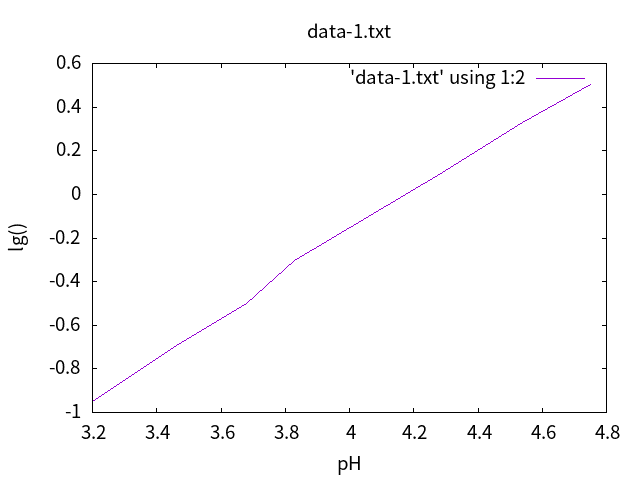
\includegraphics[width=.9\linewidth]{../img/data-1.txt.png}
\end{center}
\begin{itemize}
\item 截距为-3.951
\item 斜率为0.942
\end{itemize}
\[
pK_{a}=-\frac{-3.951}{0.942}=4.194
\]
误差:
\[
\sigma=pK_{a}\sqrt{\frac{\sigma_{A}^{2}}{A^{2}}+\frac{\sigma_{B}^{2}}{B^{2}}}=0.100
\]
\[
pK_{a}=4.194\pm 0.100
\]
\[
K_{a}=6.397\times 10^{-5}
\]
查文献得理论值为pK\textsubscript{a}=4.10,K\textsubscript{a}=7.9\texttimes{} 10\textsuperscript{-5}

相对误差为:
\[
pK_{a}: \frac{4.194-4.10}{4.10}\times 100\% =2.29\%
\]
\[
K_{a}: \frac{7.9\times 10^{-5}-6.397\times 10^{-5}}{7.9\times 10^{-5}}\times 100\%=19.0\%
\]
\item 592.20nm
\label{sec:org33fe8ec}
\begin{center}
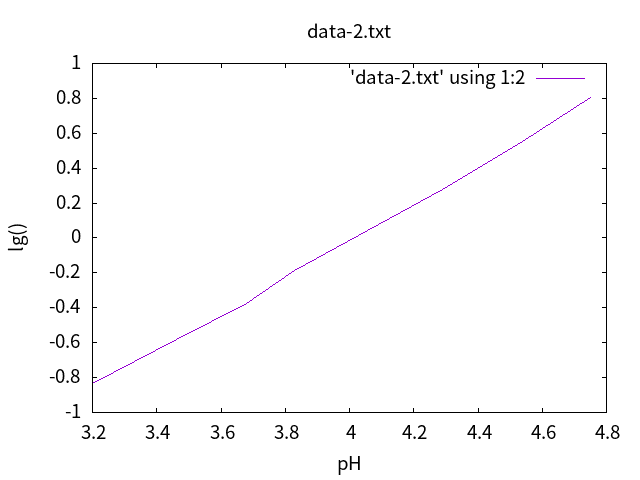
\includegraphics[width=.9\linewidth]{../img/data-2.txt.png}
\end{center}
\begin{itemize}
\item 截距为-4.242
\item 斜率为1.058
\end{itemize}
\[
pK_{a}=-\frac{-4.242}{1.058}=4.009
\]
误差:
\[
\sigma=pK_{a}\sqrt{\frac{\sigma_{A}^{2}}{A^{2}}+\frac{\sigma_{B}^{2}}{B^{2}}}=0.082
\]
\[
pK_{a}=4.009\pm 0.082
\]
\[
K_{a}=9.795\times 10^{-5}
\]
查文献得理论值为pK\textsubscript{a}=4.10,K\textsubscript{a}=7.9\texttimes{} 10\textsuperscript{-5}

相对误差为:
\[
pK_{a}: \frac{4.009-4.10}{4.10}\times 100\% =-2.22\%
\]
\[
K_{a}: \frac{7.9\times 10^{-5}-9.795\times 10^{-5}}{7.9\times 10^{-5}}\times 100\%=24.0\%
\]
\end{enumerate}
\section{实验讨论}
\label{sec:orgf1548ac}
\begin{enumerate}
\item 误差分析
\label{sec:orgfa68678}
本次实验虽然误差较小但是仍然有可以提升的空间,见下:
\begin{enumerate}
\item 贝尔-郎比定律要求入射光为单色光,但是即使是现代高精度分光光度计,也难以获得纯单色光。大多数分光光光度计只能获得近乎单色的狭窄光通带,它仍然具有复色光的性质,而复色光可导致贝尔-郎比定律的偏离,造成误差。
\item PH计的精度随着用的次数增多,精度下降,测得的PH值与书上列表中的值相差较大,每个溶液相差0.1左右,所以实验做出来的直线截距偏大,Ka偏大。
\item 比色皿光面有少量划痕,对吸光度的测定有一定的影响,从而造成误差
\item 由于测PH值及吸光度的溶液不是完全相同,尽管每次测之前都会三次润洗所用的比色皿及烧杯,仍会造成误差,一些点测得不准可能就是由这个原因造成的。
\end{enumerate}
\item 实验总结
\label{sec:org68bcd41}
\begin{enumerate}
\item 用分光光度计进行测定,用空白溶液校正零点是为了使各组溶液测出的吸光度有一个统一的基准.理论上应该使用被测溶液中不含有在测量波长处可吸收单色光的物质时所配置的溶液. 当试剂及显色剂均为无色时,可用蒸馏水作为参比溶液。对单组分溶液,使用分光光度法需要溶液遵循贝尔-郎比定律.对多组分溶液,情况比较复杂,本次实验所研究的体系是混合物中各组分的特征吸收不相重叠,即在波长λ时,只有一种物质显著吸收而其他组分可以忽略,则可只读取波长λ下测定该物质吸光度的值进行计算.
\item 测量电离常数,用紫外分光光度法可以比较准确地测定,但问题是,这种操作方法比较复杂,对实验要求比较高。采用电位法、电导法同样可以测得比较准确的结果;在用分光光度法前,可以用简单的方法先粗略地估计PKa的值:
\begin{itemize}
\item 在(25\textpm{} O.5)\textsuperscript{o}C,将弱酸和NaOH按摩尔数比1:1混合,在水溶液中进行反应。由于反应完全后[HA]一[A\textsuperscript{-}],则pKa一-pH,此时用pH计测其反应液的pH,即得粗测的pKa。\textsubscript{[3]}
\end{itemize}
\item 在本实验中,文献\textsubscript{[4]}中提到造成误差的另一个原因是PH的选泽,只有在一定PH范围内得到的数据才能有比较好的线性性,否则太酸或太碱下的数据会失去意义。
\item 溶剂的极性也会对体系产生比较大的影响\textsubscript{[5]},因而选取溶剂很关键,本实验好在溴酚蓝在水中的的溶解性很好,可以省去这方面的考虑。
\end{enumerate}
\end{enumerate}



\part{参考文献}
\label{sec:org2a32c82}
\begin{enumerate}
\item 崔献英,柯燕雄,单绍纯编。《物理化学实验》,中国科学技术大学出版社(2000年)
\item 傅献彩,沈文霞,姚天扬编。《物理化学》(第五版),高等教育出版社(2005年)
\item 《苯甲酸电离常数三种测定方法的比较》 徐雯,何风云,朱子丰 南京晓庄学院学报(JOURNAL OF NANJING XIAOZHUANC UNIVERSITY)2009年5月 第3期
\item 《紫外分光光度法测定经丙基甲基纤维素偏苯三甲酸醋的电离常数》 王文俊, 徐雅青, 邵自强 北 京 理 工 大 学 学 报Transactions of Beijing Institute of Technology 2008年1月 第28卷第1期
\item 《香荆芥酚的荧光光谱和吸收光谱研究》 李丽然,刘翠格,魏永巨光谱学与光谱分析 Spectroscopy and Spectral Analysis 2011年10月 第31卷,第10期
\item PHYSICAL CHEMISTRY   by : A.G.Whittaker, A.R.Mount \& M.R.Heal;  BIOS SCIENTIFIC PUBLISHERS LIMITED
\end{enumerate}
\part{附录: 数据处理过程}
\label{sec:orgd41b748}
\chapter{原始数据}
\label{sec:orgac06086}
\section{各组吸光度}
\label{sec:org7ad9e69}
\begin{enumerate}
\item 1
\label{sec:org836707a}
\begin{center}
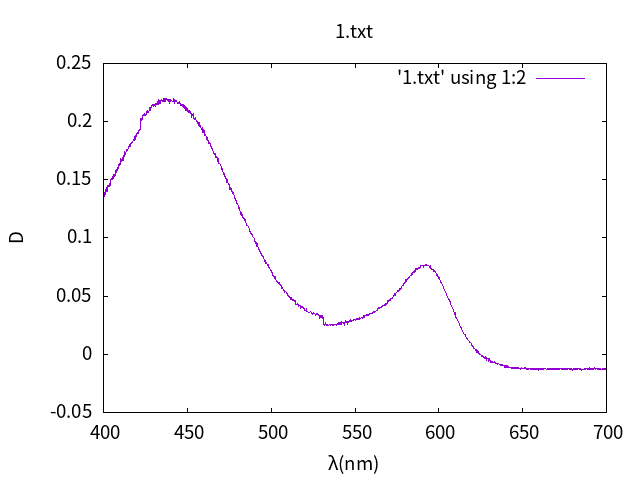
\includegraphics[width=.9\linewidth]{../img/1.txt.png}
\end{center}
\item 2
\label{sec:org3a85284}
\begin{center}
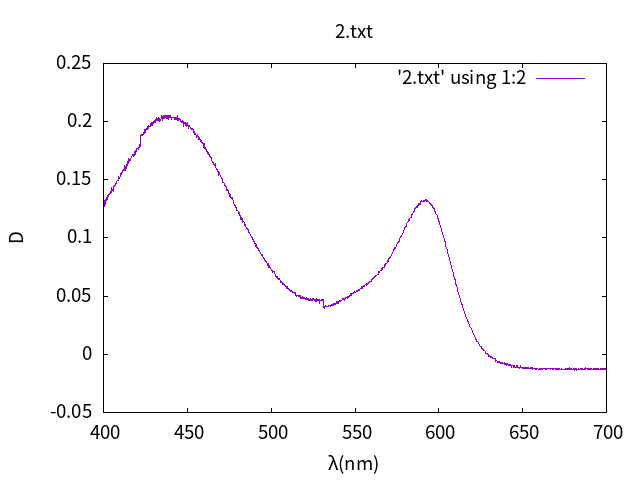
\includegraphics[width=.9\linewidth]{../img/2.txt.png}
\end{center}
\item 3
\label{sec:org43533a1}
\begin{center}
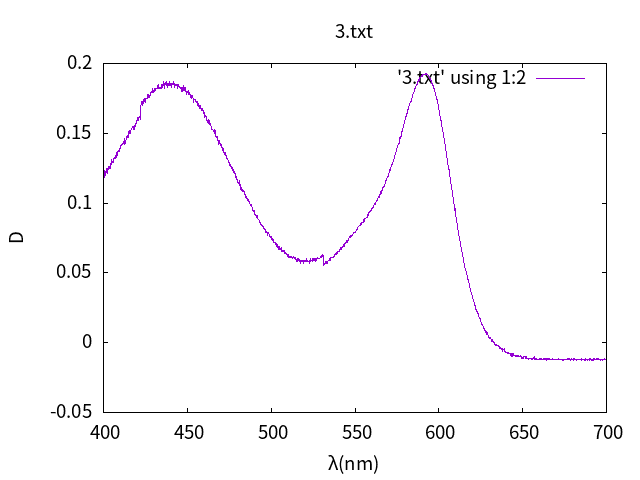
\includegraphics[width=.9\linewidth]{../img/3.txt.png}
\end{center}
\item 4
\label{sec:org1f23a86}
\begin{center}
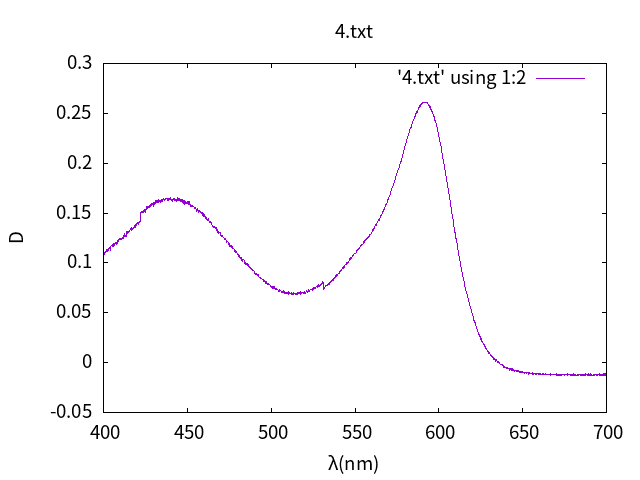
\includegraphics[width=.9\linewidth]{../img/4.txt.png}
\end{center}
\item 5
\label{sec:org818fa1a}
\begin{center}
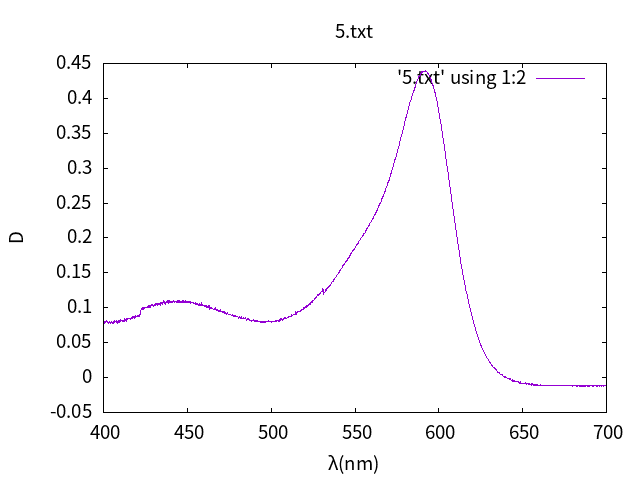
\includegraphics[width=.9\linewidth]{../img/5.txt.png}
\end{center}
\item 6
\label{sec:org3eb314f}
\begin{center}
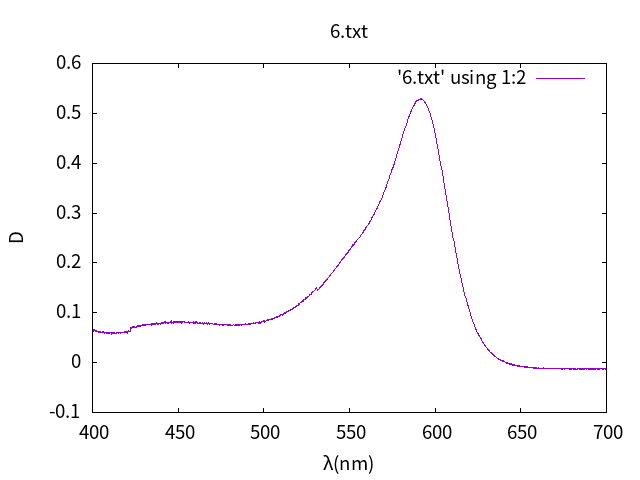
\includegraphics[width=.9\linewidth]{../img/6.txt.png}
\end{center}
\item 7
\label{sec:orgc1a17d4}
\begin{center}
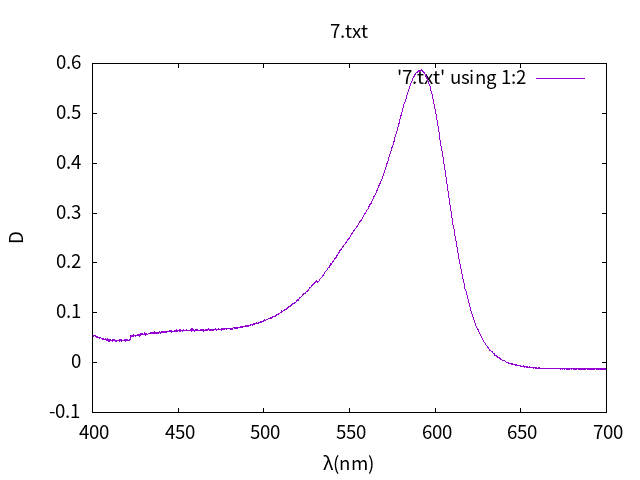
\includegraphics[width=.9\linewidth]{../img/7.txt.png}
\end{center}
\item 极酸
\label{sec:org802b35a}
\begin{center}
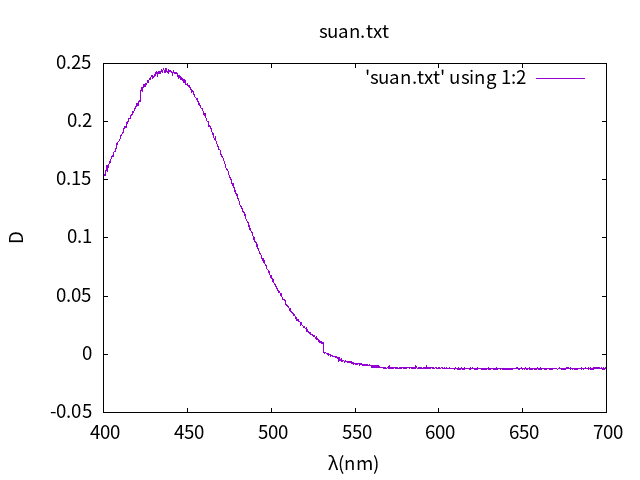
\includegraphics[width=.9\linewidth]{../img/suan.txt.png}
\end{center}
\item 极碱
\label{sec:org5ddcaae}
\begin{center}
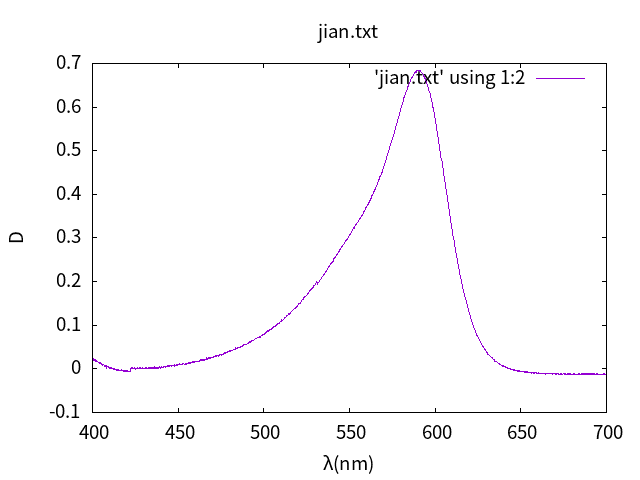
\includegraphics[width=.9\linewidth]{../img/jian.txt.png}
\end{center}
\end{enumerate}
\section{各组pH}
\label{sec:orgb0f8694}
\begin{center}
\begin{tabular}{rr}
序号 & pH\\
\hline
1 & 3.20\\
2 & 3.46\\
3 & 3.68\\
4 & 3.83\\
5 & 4.29\\
6 & 4.54\\
7 & 4.75\\
极酸 & ---\\
极碱 & ---\\
\end{tabular}
\end{center}
\chapter{数据处理}
\label{sec:org6990db6}
\section{最大吸收波长}
\label{sec:org7ca3d81}
\begin{enumerate}
\item 440nm处的峰
\label{sec:org76ad615}
\begin{center}
\begin{tabular}{rr}
序号 & 最大吸收波长\\
\hline
1 & 442.00\\
2 & 444.20\\
3 & 442.00\\
4 & 444.20\\
5 & 442.00\\
极酸 & 437.40\\
平均 & 441.97\\
6 & ---\\
7 & ---\\
极碱 & ---\\
 & \\
 & \\
\end{tabular}
\end{center}
排除掉6,7和极碱出峰不明显的组后得到该峰的波长为441.97nm

\item 590nm处的峰
\label{sec:org5579f9e}
\begin{center}
\begin{tabular}{rr}
序号 & 最大吸收波长\\
\hline
1 & 592.80\\
2 & 592.80\\
3 & 592.80\\
4 & 593.00\\
5 & 592.20\\
6 & 591.80\\
7 & 591.80\\
极碱 & 591.20\\
平均 & 592.30\\
极酸 & ---\\
\end{tabular}
\end{center}
排除掉出峰不明显的极酸,得到该峰波长为592.30nm
\end{enumerate}

\section{各组吸光度-pH}
\label{sec:org7be39ef}

\begin{enumerate}
\item 442.00nm
\label{sec:org1d30bc0}
\begin{center}
\begin{tabular}{rrrrrr}
序号 & 吸光度1(442.00nm) & pH & (1)ln(D-D\textsubscript{1})/(D\textsubscript{2}-D) & (1)pK\textsubscript{a} & lg\\
\hline
1 & 0.220 & 3.20 & -2.188 & 5.388 & -0.950\\
2 & 0.204 & 3.46 & -1.599 & 5.059 & -0.694\\
3 & 0.187 & 3.68 & -1.155 & 4.835 & -0.502\\
4 & 0.165 & 3.83 & -0.699 & 4.529 & -0.304\\
5 & 0.111 & 4.29 & 0.236 & 4.054 & 0.102\\
6 & 0.082 & 4.54 & 0.757 & 3.783 & 0.329\\
7 & 0.063 & 4.75 & 1.155 & 3.595 & 0.502\\
极酸 & 0.244 & --- &  &  & \\
极碱 & 0.006 & --- &  &  & \\
 &  &  &  &  & \\
\end{tabular}
\end{center}

\begin{center}
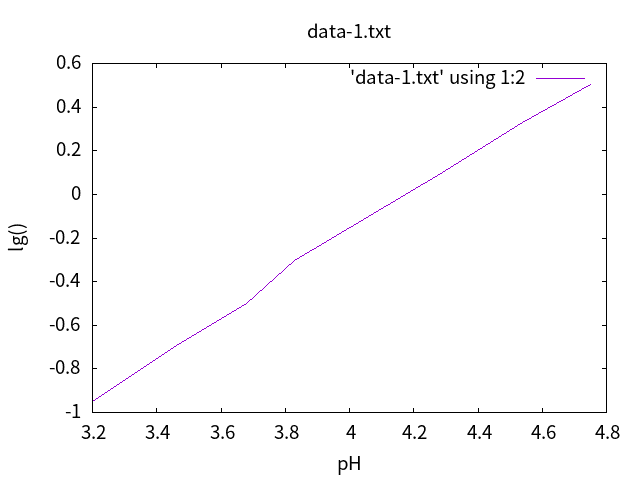
\includegraphics[width=.9\linewidth]{../img/data-1.txt.png}
\end{center}
     拟合结果:
\begin{verbatim}
iter      chisq       delta/lim  lambda   k             b            
   0 4.5236452061e+00   0.00e+00  9.75e+00    2.435614e+00  -9.767469e+00
   1 3.8539344331e+00  -1.74e+04  9.75e-01    2.330494e+00  -9.494374e+00
   2 7.5826190228e-02  -4.98e+06  9.75e-02    1.133254e+00  -4.716064e+00
   3 2.6383711206e-03  -2.77e+06  9.75e-03    9.423133e-01  -3.952324e+00
   4 2.6381845581e-03  -7.07e+00  9.75e-04    9.420080e-01  -3.951103e+00
   5 2.6381845581e-03  -1.58e-09  9.75e-05    9.420080e-01  -3.951103e+00
iter      chisq       delta/lim  lambda   k             b            

After 5 iterations the fit converged.
final sum of squares of residuals : 0.00263818
rel. change during last iteration : -1.57811e-14

degrees of freedom    (FIT_NDF)                        : 5
rms of residuals      (FIT_STDFIT) = sqrt(WSSR/ndf)    : 0.0229703
variance of residuals (reduced chisquare) = WSSR/ndf   : 0.000527637

Final set of parameters            Asymptotic Standard Error
=======================            ==========================
k               = 0.942008         +/- 0.01627      (1.728%)
b               = -3.9511          +/- 0.0651       (1.648%)

correlation matrix of the fit parameters:
#                k      b      
k               1.000 
b              -0.991  1.000 

\end{verbatim}
\[
lg=0.942*pH-3.951
\]
\begin{itemize}
\item 截距为-3.951
\item 斜率为0.942
\end{itemize}
\[
pK_{a}=-\frac{-3.951}{0.942}=4.194
\]
误差:
\[
\sigma=pK_{a}\sqrt{\frac{\sigma_{A}^{2}}{A^{2}}+\frac{\sigma_{B}^{2}}{B^{2}}}=0.100
\]
\[
pK_{a}=4.194\pm 0.100
\]
\[
K_{a}=6.397\times 10^{-5}
\]
查文献得理论值为pK\textsubscript{a}=4.10,K\textsubscript{a}=7.9\texttimes{} 10\textsuperscript{-5}

相对误差为:
\[
pK_{a}: \frac{4.194-4.10}{4.10}\times 100\% =2.29\%
\]
\[
K_{a}: \frac{7.9\times 10^{-5}-6.397\times 10^{-5}}{7.9\times 10^{-5}}\times 100\%=19.0\%
\]
\item 592.20nm
\label{sec:org9fb717c}
\begin{center}
\begin{tabular}{rrrrrr}
序号 & 吸光度2(592.20nm) & pH & (2)ln(D-D\textsubscript{1})/(D\textsubscript{2}-D) & (2)pK\textsubscript{a} & lg\\
\hline
1 & 0.076 & 3.20 & -1.925 & 5.125 & -0.836\\
2 & 0.132 & 3.46 & -1.335 & 4.795 & -0.580\\
3 & 0.192 & 3.68 & -0.870 & 4.550 & -0.378\\
4 & 0.261 & 3.83 & -0.426 & 4.256 & -0.185\\
5 & 0.440 & 4.29 & 0.637 & 3.653 & 0.277\\
6 & 0.528 & 4.54 & 1.274 & 3.266 & 0.553\\
7 & 0.586 & 4.75 & 1.861 & 2.889 & 0.808\\
极酸 & -0.012 & --- &  &  & \\
极碱 & 0.679 & --- &  &  & \\
 &  &  &  &  & \\
 &  &  &  &  & \\
\end{tabular}
\end{center}
\begin{center}
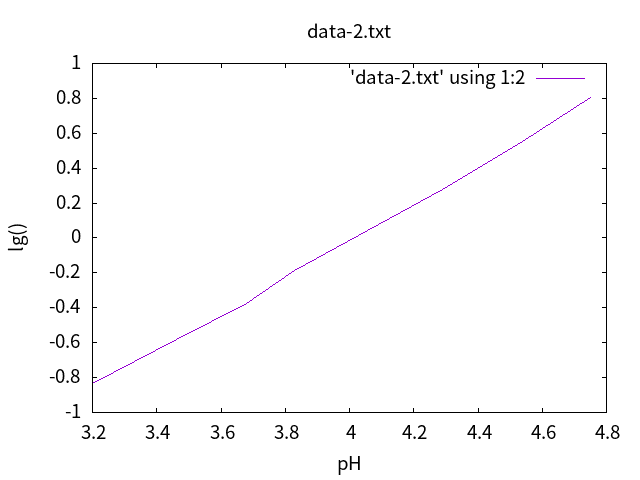
\includegraphics[width=.9\linewidth]{../img/data-2.txt.png}
\end{center}
拟合结果:
\begin{verbatim}
iter      chisq       delta/lim  lambda   k             b            
   0 2.2661113465e-01   0.00e+00  3.86e+00    9.420080e-01  -3.951103e+00
   1 1.9366690759e-02  -1.07e+06  3.86e-01    9.667043e-01  -3.889419e+00
   2 2.6711626574e-03  -6.25e+05  3.86e-02    1.045345e+00  -4.192349e+00
   3 2.3643612896e-03  -1.30e+04  3.86e-03    1.057711e+00  -4.241783e+00
   4 2.3643605040e-03  -3.32e-02  3.86e-04    1.057731e+00  -4.241862e+00
iter      chisq       delta/lim  lambda   k             b            

After 4 iterations the fit converged.
final sum of squares of residuals : 0.00236436
rel. change during last iteration : -3.32263e-07

degrees of freedom    (FIT_NDF)                        : 5
rms of residuals      (FIT_STDFIT) = sqrt(WSSR/ndf)    : 0.0217456
variance of residuals (reduced chisquare) = WSSR/ndf   : 0.000472872

Final set of parameters            Asymptotic Standard Error
=======================            ==========================
k               = 1.05773          +/- 0.01541      (1.457%)
b               = -4.24186         +/- 0.06163      (1.453%)

correlation matrix of the fit parameters:
#                k      b      
k               1.000 
b              -0.991  1.000 

\end{verbatim}
\[
lg=1.058*pH-4.242
\]
\begin{itemize}
\item 截距为-4.242
\item 斜率为1.058
\end{itemize}
\[
pK_{a}=-\frac{-4.242}{1.058}=4.009
\]
误差:
\[
\sigma=pK_{a}\sqrt{\frac{\sigma_{A}^{2}}{A^{2}}+\frac{\sigma_{B}^{2}}{B^{2}}}=0.082
\]
\[
pK_{a}=4.009\pm 0.082
\]
\[
K_{a}=9.795\times 10^{-5}
\]
查文献得理论值为pK\textsubscript{a}=4.10,K\textsubscript{a}=7.9\texttimes{} 10\textsuperscript{-5}

相对误差为:
\[
pK_{a}: \frac{4.009-4.10}{4.10}\times 100\% =-2.22\%
\]
\[
K_{a}: \frac{7.9\times 10^{-5}-9.795\times 10^{-5}}{7.9\times 10^{-5}}\times 100\%=24.0\%
\]
\end{enumerate}
\end{document}
